%TODO : rajouter images

\chapter{Graphical User Interface}

In this work a graphical user interface was developed to simplify the accessibility to the software by non initiated users. A very simple but ergonomic interface was choosen. The aim was to deal as best as possible with the two problems, (the picture from a moving train and the blur item take by a camera) without spending too much time on graphical details of the GUI.


The graphical user interface is open by calling the function GUI.m. Firstly the user is invited to choose the kind of problem in a menu bar.


\section{Train}

The user can choose an image. Two cases are possibles: either he wants to artificially blur it or deblurring it.

\begin{figure}[h]
\centering
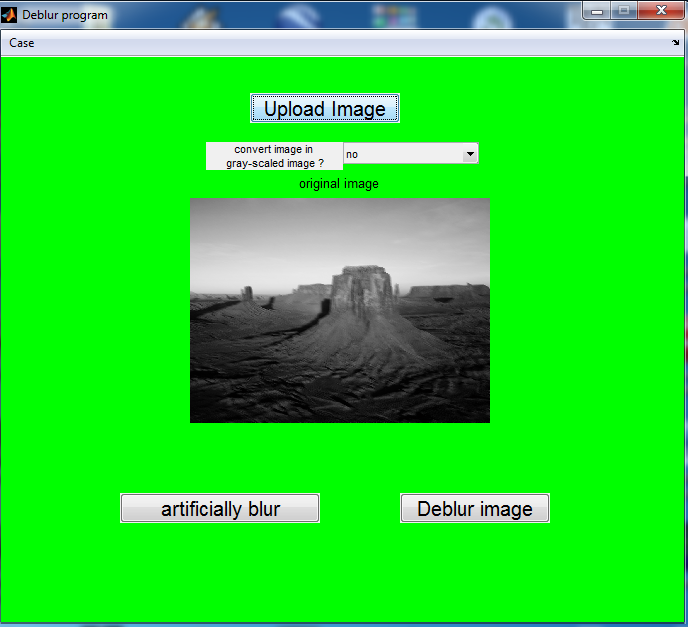
\includegraphics[{width=0.4 \textwidth}]{../Images/GUI/train.png}
\label{fig:GUItrain}
\caption{principal screen for the case of train}
\end{figure} 

If he chooses to blur artificially the image(useful for validation tests), a new window is opened and the user can enter an angle and a length of blur. The resulting blurred image (after pressing "GO !") can then be deblurred, which brings us to the second possibility. It's also possible for the user to save the blurred image.

\begin{figure}[h]
\centering
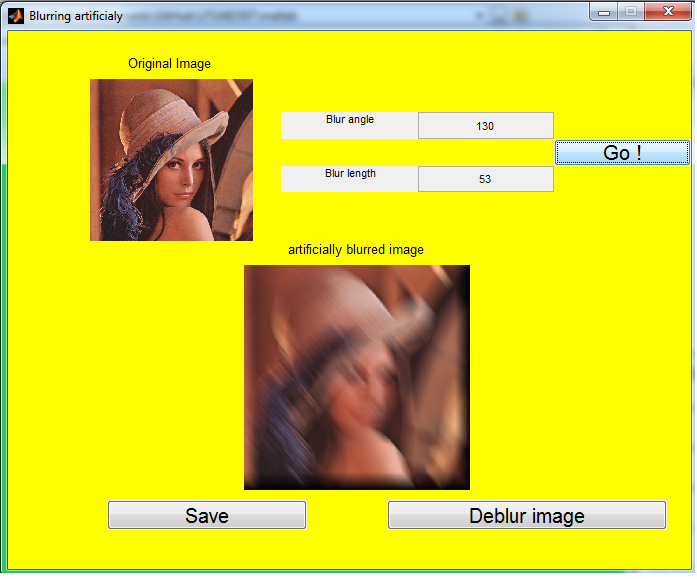
\includegraphics[{width=0.4 \textwidth}]{../Images/GUI/trainBlur.png}
\label{fig:GUItrainBlur}
\caption{Artificial blur with the GUI}
\end{figure} 

In case the user chooses to deblur the original image (or the artificially blurred one), a new window is opened. In this one, it's possible to choose or not to compress the photo to deblur (in order to accelerate the deconvolution,  as mentioned in our supplementary item) and deblurring method  (which will allow subsequently compare different results depending on the method used). The button "GO !" launches deblurring. The deblurred image can finally be save in a file.

\begin{figure}[h]
\centering
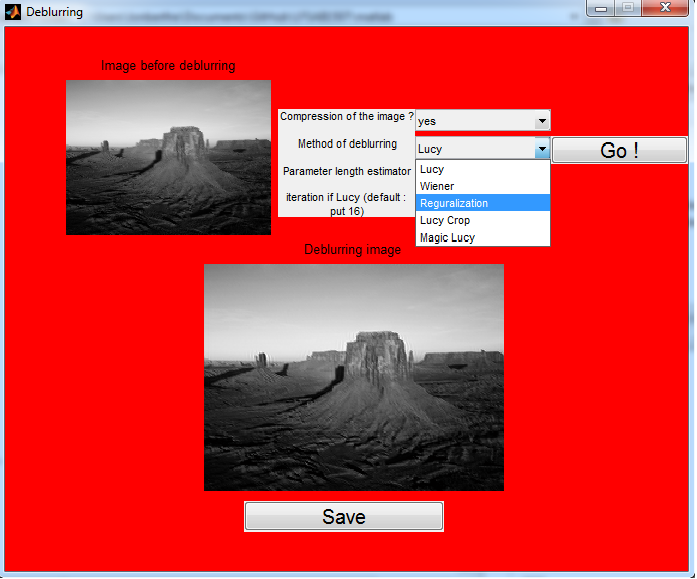
\includegraphics[{width=0.4 \textwidth}]{../Images/GUI/trainDeblur.png}
\label{fig:GUItrainDeblur}
\caption{Deblur with the GUI}
\end{figure} 

\section{Camera video}

The user is prompted to select the folder containing the serie of images that we want to make the background (only one image in the folder if the background is known). The calculated background can then be optionally recorded.
Then, the user selects the folder of all images to deblur (with blurred foreground) and for each of them, the deblurred image is displayed next to the original one. Simultaneously, the background is updated taking into account any changes (new item, change brightness, ...).

\begin{figure}[h]
\centering
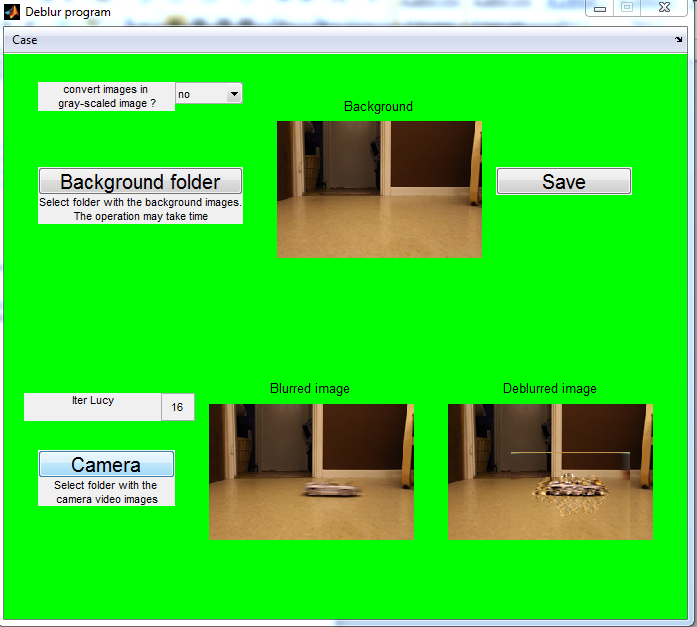
\includegraphics[{width=0.4 \textwidth}]{../Images/GUI/camera.png}
\label{fig:GUIcam}
\caption{Case of the camera video with the GUI}
\end{figure} 

\chapter{Specifications}

\section{Train}

\paragraph{Problem}
A picture is taken from a moving train. We have to deblur the image with or without the knowledge of the speed.

\paragraph{Assumptions}
1. camera is parallel to the train 2. speed is constant during the short period of time when the picture is taken 3. all the subjects of the scene are approximatively in the same vertical plane: the distance to the camera is constant

\paragraph{Input}
1. the blurred image $G$. The pixels take values from $0$ to $255$ as we use a 8bits representation. If $G$ a is grey-scaled image, $G \in \mathbb{R}^{M \times N}$. If $G$ is a coloured image, $G \in \mathbb{R}^{M \times N \times 3}$. 2. If the train's speed is known: a. speed $v$ b. opening angle $\phi$ of the camera c. average distance $\eta$ from the camera to the scene c. exposure time $\Delta t$ of the camera 

\paragraph{Output}
deblurred image of $F$

\paragraph{Performance}
A criterion of quality computes the amount of blur in an image. Ideally, the criterion should be a no-referential blur metric, that means that it doesn't depend upon the original image. The value that this method returns is then an absolute value associated with the image.

\section{Security Camera}

\paragraph{Problem}
A picture is taken by a security camera. We have to deblur a part of the image where a subject is moving. We also have a sample of statistical images taken without the subject.

\paragraph{Assumptions}
1. Camera is fixed 2. the luminance of the images of the sample don't vary too much

\paragraph{Input}
1. the blurred image $G$. The pixels take values from $0$ to $255$ as we use a 8bits representation. If $G$ a is grey-scaled image, $G \in \mathbb{R}^{M \times N}$. If $G$ is a coloured image, $G \in \mathbb{R}^{M \times N \times 3}$. 2. Sample of statistical images taken without the subject that have the same dimensions as $G$. 3. criterion of the user: a. quick processing at the expense of a good quality. Example: the client is in charge of the security in a bank and has a camera that takes pictures every second. He would like to have a usable version of those pictures on his screen. So the quality of the images doesn't matter, he only needs an idea of what's going on. b. high quality of deblurring, no matters the time spend in it. Example: the client needs a sharp image of the people's faces to determine their exact identity.

\paragraph{Output}
The ouput is the deblurred image according to the criterion given by the user.

\paragraph{Performance}
If the user chose for quality criterion, we apply the same method as for train. If he chose for the quickness criterion, we compute the time our algorithm takes and optimise it. 

\chapter{Logbook}
\section{Introduction}

Throughout the project, we have maintained a logbook including the distribution of work among group members. This well reflects the work that remains to be done and helps to improve the general organization of the project.

\section{Work Distribution}

\subsection*{Week 1 : Mathematical Modelisation}
\paragraph{Benoît} Camera
\paragraph{Arnaud} Camera
\paragraph{Geoffroy} Train
\paragraph{Jonathan} Train

\subsection*{Week 2 : Mathematical Modelisation}
\paragraph{Benoît} Train
\paragraph{Arnaud} Train
\paragraph{Geoffroy} Camera
\paragraph{Jonathan} Camera

\subsection*{week 3 : Specifications}
\paragraph{Benoît} Inputs for both situations
\paragraph{Arnaud} Outputs for both situations
\paragraph{Geoffroy} Blur metric
\paragraph{Jonathan} Assumptions for both situations

\subsection*{Week 4}
\paragraph{Benoît} some research about Lucy-Richardson algorithm + angle estimation
\paragraph{Arnaud} supplementary item + angle estimation
\paragraph{Geoffroy} comments on modelisation and specifications of group + length estimation
\paragraph{Jonathan} working plan + length estimation

\subsection*{Week 5}
\paragraph{Benoît} lucy-richardson + Radon
\paragraph{Arnaud} angle estimation of PSF with Radon
\paragraph{Geoffroy} no referential blur metric
\paragraph{Jonathan} length estimation of PSF with cepstrum

\subsection*{Week 6}
\paragraph{Benoît} slides lucy richardson
\paragraph{Arnaud} slides angle estimation
\paragraph{Geoffroy} slides blur metric 
\paragraph{Jonathan} slides length estimation

\subsection*{Week 7}
\paragraph{Benoît} lucy-richardson improved
\paragraph{Arnaud} Wiener algorithm
\paragraph{Geoffroy} angle estimation with Gabor
\paragraph{Jonathan} GUI

\subsection*{Week 8}
\paragraph{Benoît} making background image
\paragraph{Arnaud} compression
\paragraph{Geoffroy} data images for testing
\paragraph{Jonathan} GUI

\subsection*{Week 9}
\paragraph{Benoît} tests lucy richardson
\paragraph{Arnaud} compression
\paragraph{Geoffroy} regularization
\paragraph{Jonathan} GUI

\subsection*{Week 10}
\paragraph{Benoît} test angle estimators
\paragraph{Arnaud} tests wiener
\paragraph{Geoffroy} test length estimator
\paragraph{Jonathan} detecting foreground

\subsection*{Week 11}
\paragraph{Benoît} report: angle estimation with radon, length estimation with cepstrum, deconvolution with lucy, foreground estimation with cam
\paragraph{Arnaud} report: conclusion, Wiener train, Wiener camera, regularization, show direct resolution matrix is useless
\paragraph{Geoffroy} report: detection foreground - background: matlab, angle estimation with Gabor, nsr estimation, mathematical formulation, specifications
\paragraph{Jonathan} report: GUI, comparison of results, background estimation for camera

\subsection*{Week 12}
\paragraph{Benoît} report: angle estimation with radon, length estimation with cepstrum, deconvolution with lucy, foreground estimation with cam
\paragraph{Arnaud} report: conclusion, Wiener train, Wiener camera, regularization, show direct resolution matrix is useless
\paragraph{Geoffroy} report: detection foreground - background: matlab, angle estimation with Gabor, nsr estimation, mathematical formulation, specifications
\paragraph{Jonathan} report: GUI, comparison of results, background estimation for camera


\chapter{Codes}

\section{PSF estimation}
\matlabcode{angle_estimator_Gabor}{}
\matlabcode{angle_estimator}{}
\matlabcode{direct}{}
\matlabcode{length_estimator}{}
\matlabcode{oneway_psf}{}
\matlabcode{robust_angle_estimator}{}

\section{Train}
\matlabcode{blur}{Blur it.}
\matlabcode{deblur}{}
\matlabcode{testBlurDeblur}{}

\section{Camera}
\matlabcode{blur_cam}{}
\matlabcode{cam}{}
\matlabcode{deblur_cam}{}
\matlabcode{testCam}{}

\section{Utils}
\matlabcode{argmax}{}
\matlabcode{biggest_square}{}
\matlabcode{blurmetric}{}
\matlabcode{compression}{}
\matlabcode{flood_fill}{}
\matlabcode{max_coord_mat}{}
\matlabcode{mse}{}
\matlabcode{plothot}{}
\matlabcode{save_image}{}
\matlabcode{squareborder}{}

\section{Background estimation}
\matlabcode{DetectBackgroundColor}{}
\matlabcode{DetectBackground}{}
\matlabcode{UpdateBackgroundColor}{}
\matlabcode{UpdateBackground}{}

\section{Deconvolution methods}
\matlabcode{lucy}{This code is inspired from the code of the Lucy-Richardson code in wikipedia written by G3aj of the University College London and modified by a user with IP 82.16.146.178.}
\matlabcode{nsrEstimation}{}

\section{GUI}
\matlabcode{GUICameravideo}{}
\matlabcode{GUITrain}{}
\matlabcode{GUI}{}
